%%%%%%%%%%%%%%%%%%%%%%%%%%%%%%%%%%%%%%%%%%%%%%%%%%%%%%%%%%%%%%%%%%%%%%%%
%                                                                      %
%     File: Thesis_Implementation.tex                                  %
%     Tex Master: Thesis.tex                                           %

%%%%%%%%%%%%%%%%%%%%%%%%%%%%%%%%%%%%%%%%%%%%%%%%%%%%%%%%%%%%%%%%%%%%%%%%

\chapter{Implementation}
\label{chapter:implementation}

\section{Overview}
\label{section:overview}

This chapter describes the implementation details of the Binary Level Serialization, Receiver and Compliance, Message Transportation and Deployment. This chapter also gives experimental examples about new implementation to show that solution works in practice and that is better than XML or JSON regarding data binding and decoupling.

%%%%%%%%%%%%%%%%%%%%%%%%%%%%%%%%%%%%%%%%%%%%%%%%%%%%%%%%%%%%%%%%%%%%%%%%
\section{Binary Level Serialization}
\label{section:binaryLevelSerialization}

In this section, the implementation of the Binary level serialization will be presented. As in previous chapters, explained advantages of binary comparing to text-based solutions, it will be showed with some experimentation.

Computer languages have their own object types and special serialization algorithms for their object types, so when you are working with same language you can easily serialize an object and deserialize it back easily with other application which is written by same language.

When starting to work with different computer languages and their object types, most probably you have problem with serialization. You cannot use standard Java or .Net(C\#) object serialization, because different program languages use different algorithms  for serialization, that's why you’ll run into the problem with serialization. Let's explain that with a simple example. For example simple Person object such as in Listing ~\ref{lst:javaperson} has a binary representation which is not the same in .Net(Table \ref{tab:netserilazitaon}) and Java(Table \ref{tab:javaserilazitaon}).\\

\begin{lstlisting}[caption=Person Object, label=lst:javaperson]
  public class Person
  {
       public String name;
       public int age;
  }
\end{lstlisting}
Because both Java and .Net has different algorithms to serialize and deserialize their object classes and they are unaware of each other. The unique solution for that problem is avoid using standard serialization libraries for Java and .Net.
\begin{table}[]
\centering
\begin{tabular}{lllllllllllllll}
0   & 1   & 0   & 0   & 0   & 255 & 255 & 255 & 255 & 1   & 0   & 0   & 0   & 0   & 0  \\
0   & 0   & 12  & 2   & 0   & 0   & 0   & 73  & 83  & 101 & 114 & 105 & 97  & 108 & 105\\
122 & 97  & 116 & 105 & 111 & 110 & 32  & 116 & 101 & 115 & 116 & 44  & 32  & 86  & 101\\
114 & 115 & 105 & 111 & 110 & 61  & 49  & 46  & 48  & 46  & 48  & 46  & 48  & 44  & 32 \\
67  & 117 & 108 & 116 & 117 & 114 & 101 & 61  & 110 & 101 & 117 & 116 & 114 & 97  & 108\\
44  & 32  & 80  & 117 & 98  & 108 & 105 & 99  & 75  & 101 & 121 & 84  & 111 & 107 & 101\\
110 & 61  & 110 & 117 & 108 & 108 & 5   & 1   & 0   & 0   & 0   & 25  & 83  & 101 & 114\\
105 & 97  & 108 & 105 & 122 & 97  & 116 & 105 & 111 & 110 & 95  & 116 & 101 & 115 & 116\\
46  & 80  & 101 & 114 & 115 & 111 & 110 & 2   & 0   & 0   & 0   & 21  & 60  & 110 & 97 \\
109 & 101 & 62  & 107 & 95  & 95  & 66  & 97  & 99  & 107 & 105 & 110 & 103 & 70  & 105\\
101 & 108 & 100 & 20  & 60  & 97  & 103 & 101 & 62  & 107 & 95  & 95  & 66  & 97  & 99 \\
107 & 105 & 110 & 103 & 70  & 105 & 101 & 108 & 100 & 1   & 0   & 8   & 2   & 0   & 0  \\
0   & 6   & 3   & 0   & 0   & 0   & 4   & 74  & 111 & 104 & 110 & 32  & 0   & 0   & 0  \\
11  &     &     &     &     &     &     &     &     &     &     &     &     &     &    \\
\end{tabular}
\caption[.Net Serialization Person Object]{.Net Serialization Person Object}
\label{tab:netserilazitaon}
\end{table}

\begin{table}[]
\centering
\begin{tabular}{lllllllllllllll}
  -84 & -19 & 0   & 5  & 115 & 114 & 0   & 23   & 106 & 97  & 118 & 97  & 97  & 112  & 112 \\
  108 & 105 & 99  & 97 & 116 & 105 & 111 & 110  & 55  & 46  & 80  & 101 & 114 & 115  & 111 \\
  110 & 79  & -70 & 94 & 85  & -31 & -32 & -110 & 90  & 2   & 0   & 2   & 73  & 0    & 3 \\
  97  & 103 & 101 & 76 & 0   & 4   & 110 & 97   & 109 & 101 & 116 & 0   & 18  & 76   & 106 \\
  97  & 118 & 97  & 47 & 108 & 97  & 110 & 103  & 47  & 83  & 116 & 114 & 105 & 110  & 103 \\
  59  & 120 & 112 & 0  & 0   & 0   & 32  & 116  & 0   & 4   & 74  & 111 & 104 & 110  &     \\
\end{tabular}
\caption[Java Serialization Person Object]{Java Serialization Person Object}
\label{tab:javaserilazitaon}
\end{table}

After that experiment, creating a common algorithm for different languages is decided to be use instead of using standard serializer for Java or .Net that both languages could understand and easily serialize or deserialize.

The binary format is always the result of serializing data in each language. Each data has a tag, which describe data type and the number of bytes that follow and the serialized content. Recovering the serialized data is simply testing the tag to find the data type and then using the number of bytes and the serialized content.

A message to be sent is an object (in Java or .Net) that provides a serialization method, which basically builds a serialized message (an array of bytes) by successively  adding each of its components, serialized. This is done by invoking the methods of the serialization class for primitive data or by recursively invoking the serialization method of structured objects that constitute the message.

Instead of every class has their own serializer class, it is implemented with idea of centralizing the “object of primitive type to a sequence of bytes” and vice-versa methods in a single class is to avoid the need for every class to have these methods. Since they are static (they receive an object and return bytes, or vice versa), they can simply be concentrated in a static class (no instances) and invoked from anywhere.

The methods to serialize, receive a primitive object (integer, Boolean, etc) and an array of bytes, returning the array of bytes with the serialized object’s bytes appended. Therefore, each serialization method grows the byte array. When the user wants to send a message, that message is an instance of a class that has a method that knows how to serialize it, by invoking the serialization methods of the static class for each of its variables.
%We will show some examples of primitive type serialization.
%\begin{figure}[!htb]
%  \centering
%  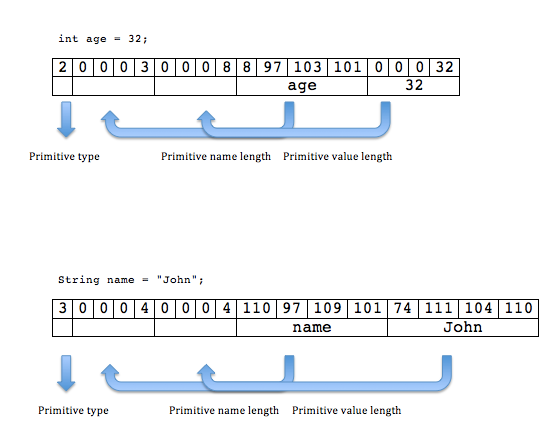
\includegraphics[width=0.9\textwidth]{Figures/binary.png}
%  \caption[Examples of primitive type serialization.]{Examples of primitive type serialization.}
%  \label{fig:examplebinary}
%\end{figure}

To examine the performance in serializing structured  data in binary and text-based data(XML,JSON), an experiment was designed using following hardware and software:
\begin{itemize}
\item 	Hardware: IMac(by Apple Inc.) with Intel Core i7 1,7 GHz and 8GB memory.
\item 	Operation System: Mac OS X version 10.11.4.
\item 	Java: version 1.8.
\end{itemize}
Current version of object serialization libraries were selected shown in the following:
\begin{itemize}
\item JAXB Serializer for XML serialization.
\item Jackson Serializer for JSON serialization.
\item OpenEXI for XML compression
\end{itemize}
The experiment was designed as follows:
\begin{itemize}
\item Ten kinds of query were prepared for weathercast provider. They were queries with ten different size of weather: 0, 100, 200, 300, 400, 500, 600, 700, 800, 900 weathercast query.
\item The serialized file was measured and the execution time was measured using System.currentTimeMillis() shown in Listing ~\ref{lst:timeserialize}.
\end{itemize}

\begin{lstlisting}[caption=Serialization program for testing, label=lst:timeserialize]
          long start = System.currentTimeMillis();
          Query q = new Query();
          for (int i = 0; i < 900; i++) {
              q.weathers.add(new Weather());
          }
          json = serialize(query);
          long end = System.currentTimeMillis();
          double time  =  (double) (end-start);
\end{lstlisting}

The avarage size of ten kinds of serialized files given in Table ~\ref{tab:binaryyy}.
\begin{table}
\centering
\begin{tabular}{ p{5.50cm} p{5.50cm} }
\toprule
\multicolumn{1}{l}{\textbf{Format}} & \textbf{Avarage (bytes)}\\
\midrule
\textbf{XML}    & 62008\\
\rowcolor{Gray}
\textbf{EXI}    & 3030\\
\textbf{JSON}   & 32036\\
\rowcolor{Gray}
\textbf{Binary} & 35984\\

\bottomrule
\end{tabular}
\caption[Sizes (in bytes) of several resource representations.]{Sizes (in bytes) of several resource representations.}
\label{tab:binaryyy}
\end{table}
\begin{figure}
    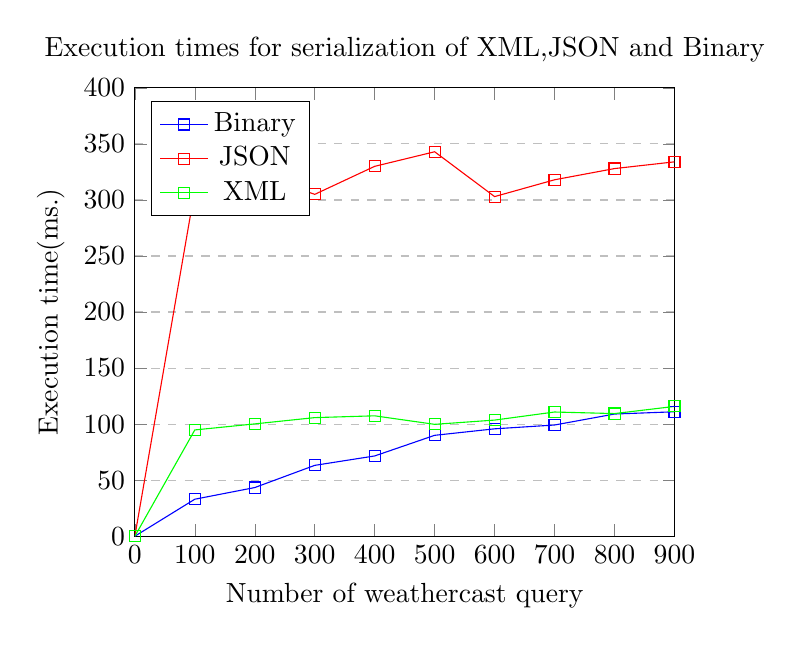
\begin{tikzpicture}
    \begin{axis}[
    title={Execution times for serialization of XML,JSON and Binary},
    xlabel={Number of weathercast query},
    ylabel={Execution time(ms.)},
    xmin=0, xmax=900,
    ymin=0, ymax=400,
    xtick={0,100,200,300,400,500,600,700,800,900},
    ytick={0,50,100,150,200,250,300,350,400},
    legend pos=north west,
    ymajorgrids=true,
    grid style=dashed,
]
\addplot[
    color=blue,
    mark=square,
    ]
    coordinates {
    (0,0)(100,33)(200,43.4)(300,63.2)(400,71.6)(500,90)(600,95.8)(700,99.2)(800,109)(900,111)
    };
   \addlegendentry{Binary}
\addplot[
    color=red,
    mark=square,
    ]
    coordinates {
   (0,0)(100,309)(200,324)(300,305)(400,330)(500,343)(600,303)(700,318)(800,328)(900,334)
    };
    \addlegendentry{JSON}
 \addplot[
    color=green,
    mark=square,
    ]
    coordinates {
   (0,0)(100,94.8)(200,100.2)(300,105.8)(400,107.4)(500,99.8)(600,103.6)(700,110.8)(800,109.4)(900,115.8)
    };
    \addlegendentry{XML}
\end{axis}
\end{tikzpicture}
\caption{Avarage Execution times for serialization of XML,JSON and Binary}
\label{fig:executiontime}
\end{figure}

From the point of the average size, the largest serialized file is obtained using XML, but EXI (Efficient XML Interchange) that use compression technology has best serialized file size when compared with others. But it does not reduce the parsing time, since text need to be recovered. On the other hand, Binary and JSON have very similar serialized file size. From the point of execution time binary serialization spends less time when compared with the others as seen in Figure~\ref{fig:executiontime}. From quantative aspects, the size of binary-based serialized data is better than XML-based and JSON-based serialization since there is no schema required and also in term of data binding, the binary-based serialization gives us big advantage with removing stub generation and DOM inspection.
%%%%%%%%%%%%%%%%%%%%%%%%%%%%%%%%%%%%%%%%%%%%%%%%%%%%%%%%%%%%%%%%%%%%%%%%

\section{Receiver and Compliance}
\label{section:compliance}

Compliance is done at the binary level, with primitive components. It is done both formal argument of the receiver method and received message. Only the components that match are assigned to the formal argument of the operation. Two partners will be able to communicate as long as the sender complies with receiver and the receiver conforms to what the sender expects and it supports all the features that the sender requires.

When a suitable operation is found, the server will complete operation and create a response for client. The system also supports optional components, which use the formal argument component if optional fields don't have value or different value. Therefore, the serialization methods in the static serialization class should include the name of the component, whether it is mandatory (with annotation), the type (encoded in the tag) and the value. Each primitive data type can have mandatory annotation. Messages sent use only with mandatory values. Serialized formal arguments can use both mandatory and non-mandatory. The receiver has always a default value for the message, so for the data that don't have mandatory annotation it will always use default value.

Let's explain that with an experiment. For that experiments there will be demonstration of 2 consumers (one developed with C\# and another with Java) and 2 providers (one developed with C\# and another with Java). General properties of 2 the consumers can be seen in Table ~\ref{tab:consumerProp}, then the properties of the providers also can be seen in Table ~\ref{tab:providerProp}


\begin{table}
\centering
\begin{tabular}{ p{5.50cm} p{5.50cm} p{5.50cm}}
\toprule
\multicolumn{1}{l}{\textbf{Device}} & \textbf{Role} & \textbf{Development technology}\\
\midrule
Mobile 1  \textbf{(Windows Mobile)}  & Consumer & C\# \\
\rowcolor{Gray}
Mobile 2  \textbf{(Android  Mobile)} & Consumer & Java \\
\bottomrule
\end{tabular}
\caption[General properties of the consumers for experiment.]{General properties of the consumers for experiment}
\label{tab:consumerProp}
\end{table}

\begin{table}
\centering
\begin{tabular}{ p{2.00cm} p{7.00cm} p{7.00cm}}
\toprule
\multicolumn{1}{l}{ } & \textbf{Cloud Server 1} & \textbf{Cloud Server 2}\\
\midrule
 \textbf{Role}                  & Provider       & Provider       \\
 \rowcolor{Gray}
 \textbf{Development technology}& .Net(C\#)      & Java            \\
 \textbf{Server technology}     & IIS 7.0 Server & Tomcat 8 Server \\
 \rowcolor{Gray}
 \textbf{Url}                   & http://csharpserverthesis.azurewebsites.net/ & http://javatomcatthesis.azurewebsites.net/ \\
\bottomrule
\end{tabular}
\caption[General properties of the providers for experiment.]{General properties of the providers for experiment}
\label{tab:providerProp}
\end{table}

Windows Mobile application (in Listing \ref{lst:wmobile}) sends 2 different query messages ({\tt Query1} as seen in Listing \ref{lst:query1} and {\tt Query2} as seen in Listing \ref{lst:query2}) to Cloud1 and Cloud2 providers. Android Mobile application (in Listing \ref{lst:andmobile}) sends a query message({\tt Query3} as seen in Listing \ref{lst:query3}) to Cloud 1 and Cloud 2 providers. If the receiver conforms to what the sender expects then there is compliance, the message received is partially assigned to that argument and the operation invoked.

\begin{lstlisting}[caption=Windows Mobile application, label=lst:wmobile]
  class Program
      {
          static void Main(string[] args)
          {
              Query1 q = new Query1();
              Message msg = new Message(q);
              string msgToSend = msg.Seriliaze();
              JavaWebServiceClient service = new JavaWebServiceClient();
              // Show result from server
              Console.WriteLine(" Result From Server: \n" + service.GetResult(msgToSend));
              Console.ReadLine();
          }

      }
\end{lstlisting}

\begin{lstlisting}[caption=Android Mobile application, label=lst:andmobile]
  public static void main(String[] args) throws Exception {
       final ChatClientEndpoint clientEndPoint = new ChatClientEndpoint(new URI("ws://javatomcatthesis.azurewebsites.net/JavaWebServerWebSocket-1.0/javawsendpoint"));
       clientEndPoint.addMessageHandler(new ChatClientEndpoint.MessageHandler() {
                   public void handleMessage(String message) {
                       System.out.println(message);
                   }
               });
         Query3 q = new Query3();;
         Message msg = new Message(q);
         byte[] msgToSend =  msg.SeriliazeBinary();
           clientEndPoint.sendMessage(msgToSend);
           Thread.sleep(30000);

   }
\end{lstlisting}

\begin{lstlisting}[caption=.Net provider [AvaliableMethod] notation in Receiver Class, label=lst:cserver]
  namespace CSharpWebServer.ist.enesuysal.thesis
  {
    public class Receiver
    {
        [AvaliableMethod]
        public void AvaliableMethod(Weather1 weather1){
        }
        [AvaliableMethod]
        public void AvaliableMethod(Weather2 weather2){
        }
        [AvaliableMethod]
        public void AvaliableMethod(Weather3 weather3){
        }
    }
  }
\end{lstlisting}

\begin{lstlisting}[caption=Java provider @AvaliableMethod notation in Receiver Class, label=lst:jaserver]
  package ist.enesuysal.thesis;
  public class Receiver
  {
    @AvaliableMethod
    public void AvaliableMethod(Weather4 weather4) {
    }
    @AvaliableMethod
    public void AvaliableMethod(Weather5 weather5) {
    }
    @AvaliableMethod
    public void AvaliableMethod(Weather6 weather6) {
    }
  }
\end{lstlisting}

\begin{lstlisting}[caption=Details of Query1 Object, label=lst:query1]
    public class WeatherQuery1
    {
      public String country = "Portugal";
      public String city = "Lisbon";
    }
\end{lstlisting}
\begin{lstlisting}[caption=Details of Query2 Object, label=lst:query2]
  public class WeatherQuery2
  {
    public int cityCode = 35121;
  }
\end{lstlisting}

\begin{lstlisting}[caption=Details of Query3 Object, label=lst:query3]
  public class WeatherQuery3
  {
    public double latitude = 38.736946;
    public double longitude  = -9.142685;
  }
\end{lstlisting}

Providers have operations with an input parameter of each of its operations. Operations have at most one argument, which can be structured. Matching will be done with message from consumer and input parameter of operations.  Input parameters of operations in each server can be seen in Table \ref{tab:providerinput}

\begin{table}
\centering
\begin{tabular}{ p{5.50cm} p{5.50cm}}
\toprule
\multicolumn{1}{l}{\textbf{Cloud Server 1}} & \textbf{Cloud Server 2} \\
\midrule
Weather1 (in Listing \ref{lst:weather1}) & Weather4 (in Listing \ref{lst:weather4}) \\
\rowcolor{Gray}
Weather2 (in Listing \ref{lst:weather2}) & Weather5 (in Listing \ref{lst:weather5}) \\
Weather3 (in Listing \ref{lst:weather3}) & Weather6 (in Listing \ref{lst:weather6}) \\
\bottomrule
\end{tabular}
\caption[Information about input parameter of operations in the provider for experiment.]{Information about input parameter of operations in the provider for experiment.}
\label{tab:providerinput}
\end{table}

\begin{lstlisting}[caption=Details of Weather Object, label=lst:weather1]
  public class Weather1
    {
      [Mandatory]
      public String country = "Portugal";
      [Mandatory]
      public String city = "Braga";
    }
\end{lstlisting}
\begin{lstlisting}[caption=Details of Weather2 Object, label=lst:weather2]
  public class Weather2
    {
      [Mandatory]
      public int cityCode = 35121;
      public String country = "Portugal";
      public String city = "Lisbon";
    }
\end{lstlisting}
\begin{lstlisting}[caption=Details of Weather3 Object, label=lst:weather3]
  public class Weather3
    {
      [Mandatory]
      public String country = "Portugal";
      [Mandatory]
      public String city = "Braga";
      public int cityCode = 351253;
      public double latitude = 41.530918;
      public double longitude  = -8.780565;
    }
\end{lstlisting}
\begin{lstlisting}[caption=Details of Weather4 Object, label=lst:weather4]
  public class Weather4
  {
    @Mandatory
    public String country = "Portugal";
    @Mandatory
    public String city = "Lisbon";
    public double latitude = 38.736946;
    public double longitude  = -9.142685;
  }
\end{lstlisting}
\begin{lstlisting}[caption=Details of Weather5 Object, label=lst:weather5]
  public class Weather5
  {
    @Mandatory
    public double latitude = 38.736946;
    @Mandatory
    public double longitude  = -9.142685;
  }
\end{lstlisting}
\begin{lstlisting}[caption=Details of Weather6 Object, label=lst:weather6]
  public class Weather6
  {
    @Mandatory
    public int cityCode = 35121;
  }
\end{lstlisting}

Lets start with Windows mobile application (Mobile 1); to explain compliance and conformance concepts, by providing a message with {\tt Query1} (in Listing \ref{lst:query1}) and sending it to .Net cloud provider (Cloud Server 1).
{\tt Weather1} object in Cloud 1 provider will not be mapped to {\tt Query1}, because {\tt Weather1} in Cloud 1 provider has 2 mandatory fields as seen in Listing \ref{lst:weather1} {\tt country} and {\tt city} fields do not have same value. {\tt Weather2} in Cloud 1 provider has 3 fields one mandatory other two are optional as seen in Listing \ref{lst:weather2} , since mandatory field is not in the {\tt Query1}, mapping will not be occur. {\tt Weather3} object in Cloud 1 provider also will not be mapped to {\tt Query1}, because {\tt Weather3} in Cloud 1 has 2 mandatory fields and 3 optional fields as seen in Listing \ref{lst:weather3}, but mandatory {\tt city} field does not have the same value as in {\tt city} field in {\tt Query1}. No suitable operation is found, the server will not complete operation and create a response for consumer in Cloud Server 1. Next step, let's try sending {\tt Query1} to Cloud Server 2 to check if there is any compliable operation. {\tt Weather4} object in Cloud 2 provider will be mapped to {\tt Query1} and compliance hold, because {\tt Weather4} in Cloud 2 has 2 mandatory fields and 2 optional fields as seen in Listing \ref{lst:weather4} and {\tt city} and {\tt country} fields have same value with the {\tt Query1}. The optional fields in {\tt Weather4} does not exist in {\tt Query1}, but that is not important since they are optional and they will be used with their default values.  Now suitable operation is found, the server will complete operation and create a response for client in Cloud Server 2. Now, what about when sending {\tt Query2} (in Listing) with Windows mobile application to Cloud 1 and Cloud 2 providers. {\tt Weather1} object in Cloud 1 provider will not be mapped to {\tt Query2} because {\tt Weather1} has 2 mandatory fiels and these fields are not exist in {\tt Query2}. {\tt Weather2} object in Cloud 1 provider will be mapped to {\tt Query2} because, {\tt Weather2} in Cloud 1 provider has 1 mandatory fields and 2 optional fields and {\tt cityCode} field has same value with the {\tt Query2}. The optional fields in {\tt Weather2} does not exist in {\tt Query2}, but that is not important since they are optional and they will be used with their default values. {\tt Query2} message will be complied with {\tt Weather2}, the server will complete operation and create a response for client in Cloud Server 1.

As explained above, sending {\tt Query1} message in Windows phone application will be mapped in Java weather provider and return result message after compliance. {\tt Query2} message in Windows phone application will be mapped in .Net weather provider and return result message after compliance.

The consumer does not need to be written in C\#. it can be written in Java or other language. Lets show implementation of Android phone application (Mobile 2).  This application has {\tt Query3} as seen in Listing \ref{lst:query3} and it will send that query message to Cloud 1 and Cloud 2 providers. Because of similar reasons explained before, any operation in Cloud 1 provider will not be mapped to {\tt Query3} because mandatory fields of {\tt Weather1}, {\tt Weather2} or {\tt Weather3} are not exist in {\tt Query3}. Any operation in Cloud 2 provider also will not be mapped with {\tt Query3}, because again mandatory fields of {\tt Weather4}, {\tt Weather5} or {\tt Weather6} are not exist in Query3.

The results that are explained above about partial assignment of Mobile 1 and Mobile 2 applications can be seen in Table \ref{tab:resultss} and in Table \ref{tab:resultss2}.

\begin{table}
\centering
\begin{tabular}{ p{2.00cm} p{2.00cm} p{2.00cm} p{2.00cm} p{2.00cm} p{2.00cm} p{2.00cm}}
\toprule
\multicolumn{1}{l}{}&{\textbf{Weather1}} & \textbf{Weather2} & \textbf{Weather3} & \textbf{Weather4} & \textbf{Weather5} & \textbf{Weather6} \\
\midrule
Query 1 & - & - & - & + & - & -\\
\rowcolor{Gray}
Query 2 & - & + & - & + & - & +\\
Query 3 & - & - & - & - & - & -\\
\bottomrule
\end{tabular}
\caption[Compliance and Conformance between Query message and Weather objects .]{Compliance and Conformance between Query message and Weather objects.}
\label{tab:resultss}
\end{table}

\begin{table}
\centering
\begin{tabular}{ p{2.50cm} p{2.50cm} p{2.50cm} p{2.50cm}}
\toprule
\multicolumn{1}{l}{}&{} & \textbf{Cloud Server 1} & \textbf{Cloud Server 2} \\
\midrule
Mobile 1 & Query 1 & No  & Yes\\
         & Query 2 & Yes & Yes\\
\rowcolor{Gray}
Mobile 2 & Query 3 & No  & No\\
\bottomrule
\end{tabular}
\caption[Compliance and Conformance between Cloud Servers and Mobile phones.]{Compliance and Conformance between Cloud Servers and Mobile phones.}
\label{tab:resultss2}
\end{table}

The demonstration in this section, show that provided solution is an alternative solution to XML, JSON, WSDL and REST. The example that presented here, involves compliance or conformance, that it works and that it allows changes to the client and to the server without informing both sides.

 %To clarify the compliance, the idea is to serialize the argument (only one, but it can be structured) of each operation of a service(receiving object). This acts like a default value, against which the message received is matched. A service receiving a message matches it against the argument of each operation, until it finds one, assigns the message to that argument (partial assignment) and runs the operation, returning eventually a result.

%When checking for compliance, a component in the message with the same name as a component in the operation’s argument matches it and can be assigned to it (if the message complies with the argument, as a whole). If not, it is ignored. If a component in the argument is not matched by any of the message’s components and is optional , retains the argument’s value (which acts as a default value). If all non-optional  components in the argument are matched, there is compliance, the matching components of the message are assigned to those of the argument with the same name and those that do not match are ignored. Thus the designation partial assignment.

%%%%%%%%%%%%%%%%%%%%%%%%%%%%%%%%%%%%%%%%%%%%%%%%%%%%%%%%%%%%%%%%%%%%%%%%
\section{Message Transportation}
\label{section:messageTransfer}

Transferring the array of bytes from sender to receiver requires a binary channel like Web Sockets (HTTP2) or more classical way by encoding and decoding the binary array with BASE64 and then use typical HTTP-based solutions (Web Services or REST). The classical solution is non-optimal compared to the other ones, but it is easier to implement with existent tools.

Message Transportation in this solution is done with essentially JavaScript and Web Sockets, to circumvent some of the limitations of HTTP. But also the solution supports classical way by encoding and decoding the binary array with BASE64 and then using typical HTTP-based solutions.

Web Sockets are chosen technology for implementation because they are fundamental in the efficient support for binary data removes this restriction, increases performance. They use the protocol upgrade feature of HTTP and provide a substantial degree of compatibility with existing systems. Now they are part of the HTML5 world, servers and firewalls are increasingly supporting them and remove this restriction, adds binary support and increases performance.

\begin{figure}[!htb]
  \centering
  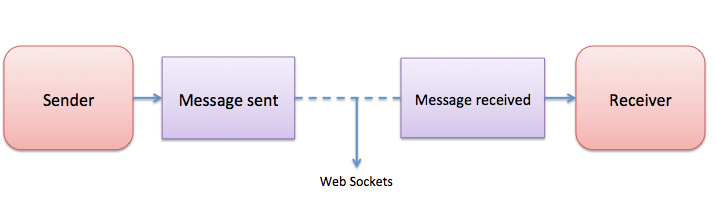
\includegraphics[width=0.5\textwidth]{Figures/websocket.png}
  \caption[Message Transportation.]{Message Transportation.}
  \label{fig:websocket}
\end{figure}

To examine the performance in HTTP-based solutions and Web Sockets, an experiment was designed using following hardware and software:

\begin{itemize}
\item 	Hardware: IMac(by Apple Inc.) with Intel Core i7 1,7 GHz and 8GB memory.
\item 	Operation System: Mac OS X version 10.11.4.
\item 	Java: version 1.8.
\end{itemize}

The experiment was designed as follows:
\begin{itemize}
\item Ten kinds of query were prepared for weathercast provider. They were queries with 6 different size of weather: 10, 100, 500, 1000, 5000, 10000 weathercast query.
\end{itemize}

\begin{figure}
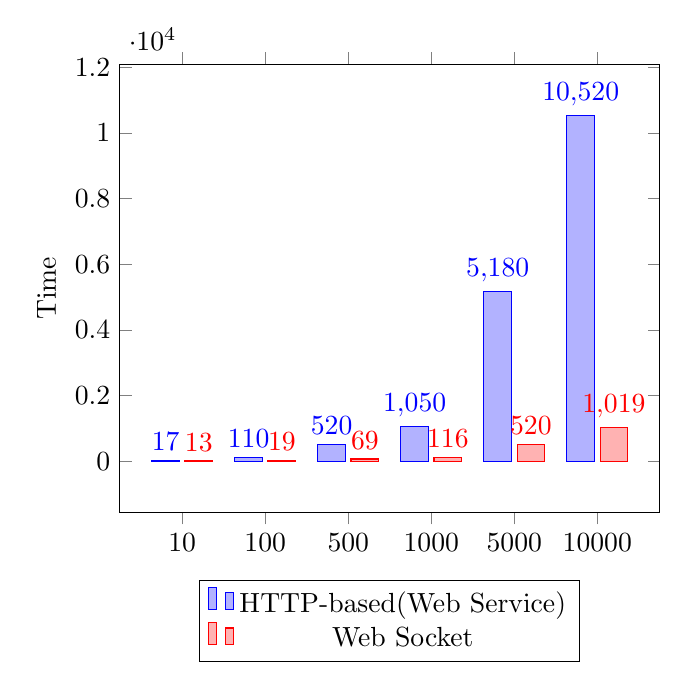
\begin{tikzpicture}
\begin{axis}[
    ybar,
    enlargelimits=0.15,
    legend style={at={(0.5,-0.15)},
      anchor=north,legend columns=1},
    ylabel={Time},
    symbolic x coords={10,100,500,1000,5000,10000},
    xtick=data,
    nodes near coords,
    nodes near coords align={vertical},
    ]
\addplot coordinates {(10,17) (100,110) (500,520) (1000,1050) (5000,5180) (10000,10520) };
\addplot coordinates {(10,13) (100,19) (500,69) (1000,116) (5000,520) (10000,1019)};

\legend{HTTP-based(Web Service),Web Socket}
\end{axis}
\end{tikzpicture}
\caption{Avarage Times(in ms) of HTTP-based solutions and WebSocket.}
\label{fig:executiontimewebsocket}
\end{figure}

\begin{table}
\centering
\begin{tabular}{ p{5.50cm}p{5.50cm} p{5.50cm} }
\toprule
\multicolumn{1}{l}{\textbf{Nb of Message}} & \textbf{Web Service(HTTP) (in ms)} & \textbf{WebSocket(in ms)}\\
\midrule
\ 10    & 17    & 13\\
\ 100   & 110   & 19\\
\ 500   & 520   & 69\\
\ 1000  & 1050  & 116\\
\ 5000  & 5180  & 520\\
\ 10000 & 10520 & 1019\\

\bottomrule
\end{tabular}
\caption[Avarage Times(in ms) of HTTP-based solutions and WebSocket.]{Times (in ms) of HTTP-based solutions and WebSocket.}
\label{tab:websov}
\end{table}

As seen in Table \ref{tab:websov} and in Figure \ref{fig:executiontimewebsocket}, there is a big difference between the HTTP-based solutions and Web Sockets. It is clear to see using Web sockets technology adds a lot difference in performance aspect. Web Sockets also removes the limitations of HTTP which adds binary support and increases performance.

%%%%%%%%%%%%%%%%%%%%%%%%%%%%%%%%%%%%%%%%%%%%%%%%%%%%%%%%%%%%%%%%%%%%%%%%

\section{Deployment}
\label{section:deployment}

The solution is developed and in two different languages that are .NET and Java. The solution is deployed to Microsoft Azure Cloud. The reason choosing Microsoft Azure Cloud instead of other providers is because Microsoft provide free access to their App Servers of Azure with student subscription account. Another reason, .Net and Java technologies can be deployed using the same platform. Microsoft Azure support Java and .Net and that's way 2 different provider will be in the same platform. The Azure application servers support Web Sockets, which is also benefit to test new solution using Web Sockets in cloud environment. .Net client can send a message to Java provider over the cloud by using Web Sockets technology and also Java client can send message to .Net provider. Using Microsoft Azure Cloud technologies allowed us to test the project in cloud environment. The characteristics of Java application server and .Net application server can be seen in Figure~\ref{fig:javaserver} and in Figure~\ref{fig:netserver}

\begin{figure}[!htb]
  \centering
  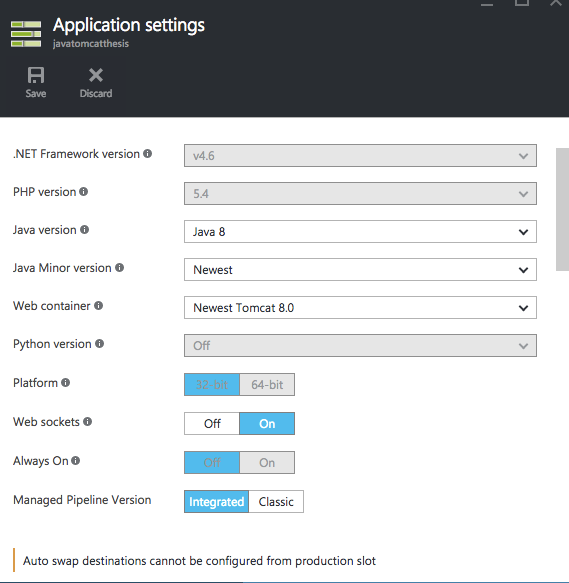
\includegraphics[width=0.7\textwidth]{Figures/javaserver.png}
  \caption[The characteristics of Java application server.]{The characteristics of Java application server.}
  \label{fig:javaserver}
\end{figure}

\begin{figure}[!htb]
  \centering
  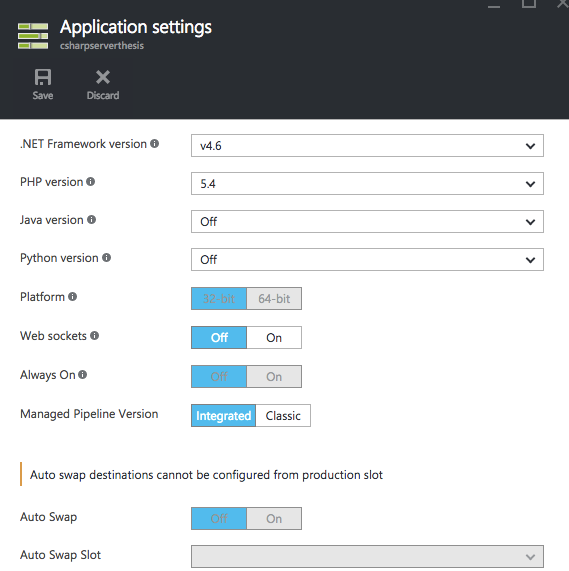
\includegraphics[width=0.7\textwidth]{Figures/dotnetserver.png}
  \caption[The characteristics of .Net application server.]{The characteristics of .Net application server.}
  \label{fig:netserver}
\end{figure}
